\chapter{Introduction}\label{ch:introduction}
In this chapter, the project is introduced and motivated. Furthermore, a brief description is presented for stereo vision and the use for it at HSA systems \todo{Måske anden formulering}. Lastly, this chapter also describes a delimitation of the project and report.\\

\section{Stereo vision introduction}
% VERSION WITH Euclid
In 280 A.D the greek mathematician Euclid described the perception  \cite{lit:historyofstereophoto}

% OLD VERSION
% Stereopsis -> binocular vision -> 
Human has the incredible ability of depth perception. This is due to our two eyes which are separated a bit from each other. Since the eyes are separated they each receive different images. These images are combined in the brain and enable us to perceive depth. This is shown on figure \ref{fig:humanviscones}. 

\begin{figure}
  \centering
  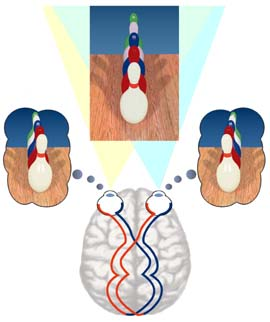
\includegraphics[height=5cm]{figures/stereovisionhuman}
  \caption{Example of human stereo vision \cite{lit:Stereovision3d}}
  \label{fig:humanviscones}
\end{figure}

This concept can be used in computer system and enable a system to perceive depth and hence distinguish between different objects.\\

Use of stereo vision:\\
Giving the ability of distinguishing between objects to a computer system gives the system the ability to perform more task. These task includes counting number of people entering pass through a secure door, enables a robot arm to interact with different objects.\\

HSA systems wish to keep an eye on packages going through their system. A strategically placed stereo vision camera will enable them to know how many and where these objects are in the system. 

\section{Motivation}
Stereo vision algorithms usually are very heavy computational wise. A high resolution real-time stereo vision can be hard to acquire. 

\section{Problem Introduction}
HSA systems wish to keep an eye on packages going through their system. A strategically placed stereo vision camera will enable them to know how many and where these objects are in the system. 
The primary objectives of this is to:
\begin{itemize}
  \item Analyze obstacles within stereo vision
  \item Analyze different stereo algorithms
  \item Design and optimize an architecture for executing stereo vision 
\end{itemize}


\section{Delimitation}
This project is mainly concerned with the design and implementation of a hardware design for a FPGA. This project will not focus on developing a new stereo vision algorithm. Obstacles and issue with stereo algorithms will not be 


\section{Report Structure and Design Process}

\begin{figure}[ht!]
  \centering
  \includegraphics[width=0.25\textwidth]{figures/A3model.jpg}
  \caption{A3 model}
  \label{fig:A3 model}
\end{figure}

The A3 methodology is a way to handle a system design. Figure 1 shows a diagram of the A3 method.  As seen it consist of 3 spaces: Application, Algorithm, and Architecture. The report will follow this structure where chapter \ref{ch:appanalysis}: Application Analysis will explore the Application space and chapter \ref{ch:req}: Requirements will contain a specification for moving into the Algorithm space. 
Chapter \ref{ch:alganalysis}: Algorithm Analysis will explore the algorithm space with the requirements as constraints. The chapter will conclude in the choice of an algorithm to be implemented on the hardware.
Chapter \ref{ch:designmet}: Design methodology will describe different methods which can be used to move from the algorithm space to the architecture space.
Chapter \ref{ch:archdesign}: Architecture Design will explore the architecture space based on the chosen algorithm. The chapter will result in a implementation of the design on the hardware platform.


